\chapter{Timeline}

The timeline is displayed at the top of each waveform group and shows the X axis scale for the group. The timeline (and
all accompanying waveform views in the group) may be zoomed by scrolling with the mouse wheel, or panned by dragging
with the left mouse button.

Unlike classical oscilloscope user interfaces, there is \emph{no relationship} between the timeline scale/position and
the duration of the acquisition. It is possible to zoom or scroll beyond the end of the acquisition (displaying empty
background with no signal) or have a deep capture in which nearly all acquired data is offscreen.

\begin{figure}[h]
\centering

\includegraphics[width=13cm]{images/timeline.png}
\caption{The timeline}
\label{timeline}
\end{figure}

TODO: talk about how to set trigger offset within acquisition, once implemented (scopehal:21, scopehal-apps:12)

Double-clicking on the timeline brings up the timebase properties dialog (Fig. \ref{timebase-properties}), which allows
the sample rate and memory depth to be configured. If multiple instruments are connected, a separate tab appears in the
dialog for each instrument.

\begin{figure}[h]
\centering
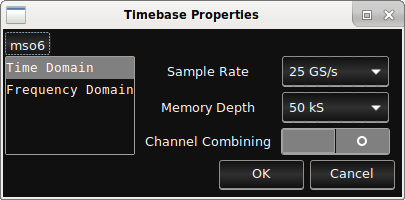
\includegraphics[width=5cm]{images/timebase-properties.png}
\caption{Timebase properties dialog}
\label{timebase-properties}
\end{figure}


Note that the timeline may occasionally show units other than time. For example, an ``eye width" measurement has X axis
units of voltage and Y axis units of time.
